%tag:000X
%label:"fig:ccStarCylinder"
%author:JeffHicks
%type:"figure"
%parent:exm:ccStarCylinder
%caption:"The symplectic structure that we choose for $\CC^*$ makes it an infinitely long cylinder."

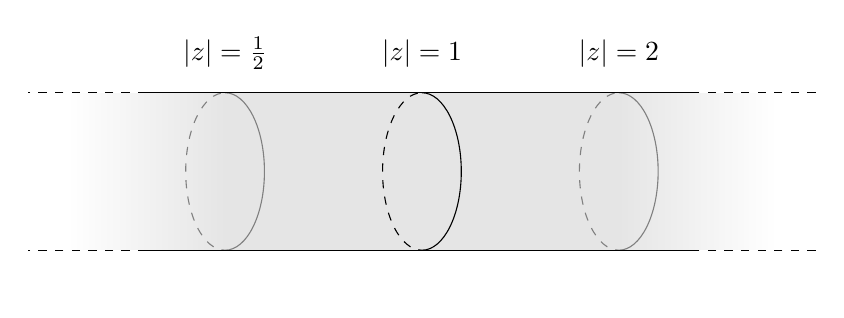
\begin{tikzpicture}

    \usetikzlibrary{fadings}
\fill[fill=gray!20, path fading = west]  (-4.5,1.5) rectangle (-2.5,-0.5);
\fill[fill=gray!20]  (-2.5,-0.5) rectangle (2.5,1.5);

\fill[fill=gray!20, path fading = east]  (4.5,1.5) rectangle (2.5,-0.5);
\begin{scope}[]

\begin{scope}[]

\clip  (0,2) rectangle (1,-1);
\draw  (0,0.5) ellipse (0.5 and 1);
\end{scope}
\begin{scope}[]

\clip  (0,2) rectangle (-1,-1);
\draw[dashed]  (0,0.5) ellipse (0.5 and 1);
\end{scope}
\end{scope}

\begin{scope}[shift={(2.5,0)}, draw=gray]

\begin{scope}[]

\clip  (0,2) rectangle (1,-1);
\draw  (0,0.5) ellipse (0.5 and 1);
\end{scope}
\begin{scope}[]

\clip  (0,2) rectangle (-1,-1);
\draw[dashed]  (0,0.5) ellipse (0.5 and 1);
\end{scope}
\end{scope}

\begin{scope}[shift={(-2.5,0)},draw=gray]

\begin{scope}[]

\clip  (0,2) rectangle (1,-1);
\draw  (0,0.5) ellipse (0.5 and 1);
\end{scope}
\begin{scope}[]

\clip  (0,2) rectangle (-1,-1);
\draw[dashed]  (0,0.5) ellipse (0.5 and 1);
\end{scope}
\end{scope}
\begin{scope}[]
\draw (-3.5,1.5) -- (3.5,1.5);
\begin{scope}[]
\draw[dashed] (-3.5,1.5) -- (-5,1.5);
\end{scope}
\begin{scope}[shift={(8.5,0)}]
\draw[dashed] (-3.5,1.5) -- (-5,1.5);
\end{scope}
\end{scope}
\begin{scope}[shift={(0,-2)}]
\draw (-3.5,1.5) -- (3.5,1.5);
\begin{scope}[]
\draw[dashed] (-3.5,1.5) -- (-5,1.5);
\end{scope}
\begin{scope}[shift={(8.5,0)}]
\draw[dashed] (-3.5,1.5) -- (-5,1.5);
\end{scope}
\end{scope}
\node at (-2.5,2) {$|z|=\frac{1}{2}$};
\node at (0,2) {$|z|=1$};
\node at (2.5,2) {$|z|=2$};
\end{tikzpicture}